\documentclass[french]{report}
\usepackage[utf8]{inputenc}
\usepackage[T1]{fontenc}
\usepackage{lmodern}
\usepackage[a4paper]{geometry}
\usepackage{babel}
\usepackage{graphicx}

\begin{document}
	\title{Functional data analysis applied to neurology}
	\author{Clément Bonvoisin, Pierre Ludmann}
	\date{30 juin 2014}
	\maketitle
	\tableofcontents

	\chapter{Introduction au problème}
	La motivation initiale de ce stage provient de la médecine, et plus particulièrement de la neurologie. Le projet, piloté par le groupe Cognac-G, vise à analyser en détail des signaux physiologiques, issus d'une expérience très simple.
	\\ \\
	Le protocole expérimental se décline comme suit :
	\begin{itemize}
		\item On place sur le patient un ensemble de capteurs : un à la tête, un à la ceinture, et un sur chaque pied. Ces capteurs sont des centrales inertielles, qui permettent une mesure de l'accélération et de la vitesse angulaire du patient.
		\item On lance l'acquisition. Pendant quelques secondes, le patient est à l'arrêt. Puis, il commence à marcher sur une dizaine de mètres, effectue un demi-tour, et fait une marche retour. Il s'arrête, et on peut alors arrêter l'acquisition.
		\item On replace alors les signaux obtenus dans un repère adapté au corps humain, formé de trois axes : l'axe antéro-postérieur, l'axe transversal (aussi appelé médio-latéral), et l'axe longitudinal (aussi appelé axe vertical) ; cf. \ref{axis}.
	\end{itemize}
	
	\begin{figure}[h]
			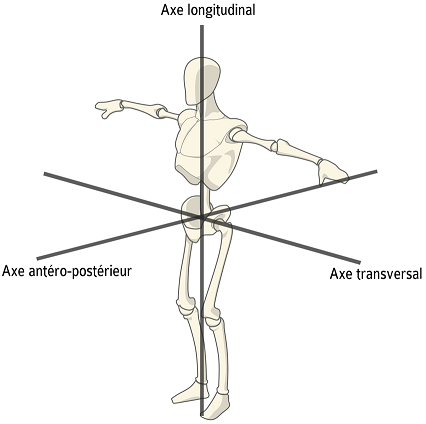
\includegraphics[scale=0.6]{axis.png}
			\caption{Repère adapté au corps humain}
			\label{axis}
	\end{figure}


	
	\chapter{Algorithme CUSUM : résolution du cas d'une seule rupture}
	
	\chapter{Cas de plusieurs ruptures : implémentation dichotomique}
	
	\chapter{Cas de plusieurs ruptures : implémentation par fenêtres}
	
	\chapter{Évaluation des performances}
	
	\chapter{Conclusion}
\end{document}
